TODO: sostituire con introduzione (tipo quella del progetto vecchio)

\begin{figure}
	\centering
	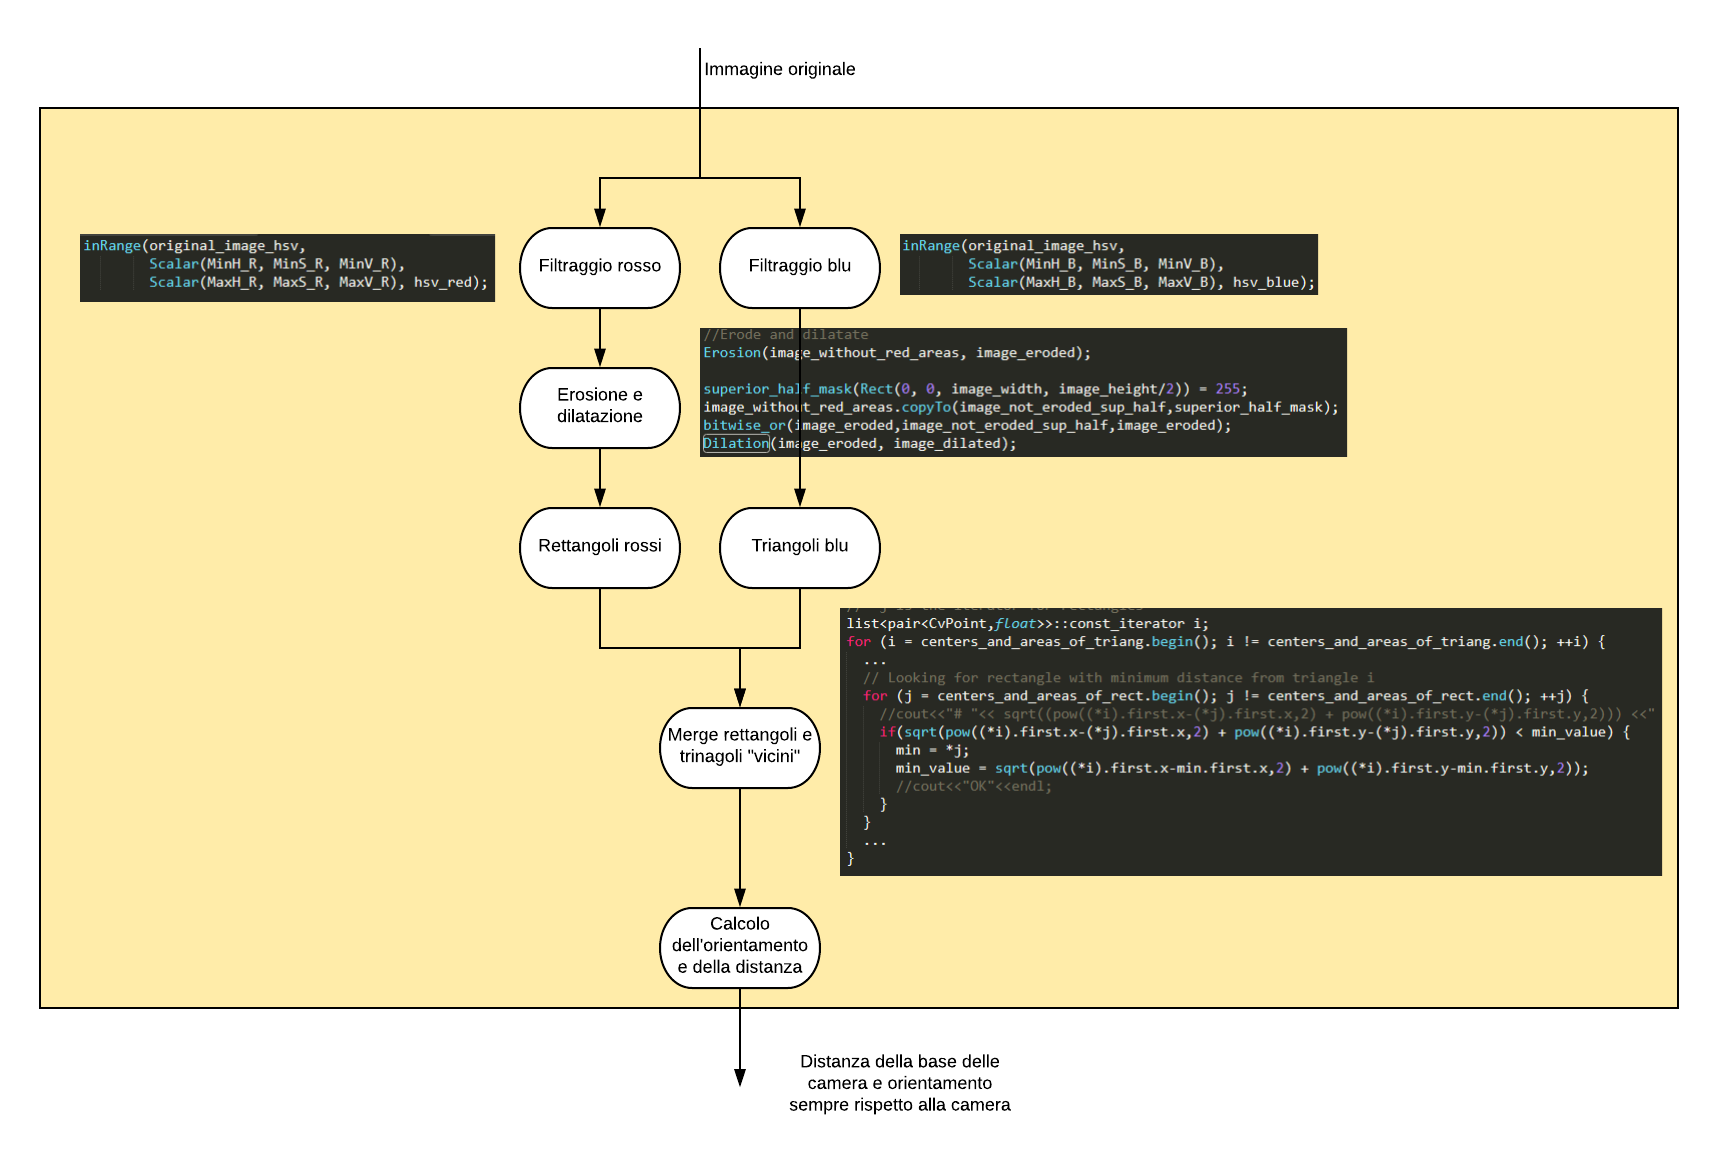
\includegraphics[width=\textwidth]{Immagini/CodeStructure.png}
	\caption{Struttura del codice}
	\label{fig:CodeStructure}
\end{figure}

Obbiettivo: andare a implementare sistema di \textit{visual navigation} per la base robotica in figura ~\ref{fig:BaseRobotica}.

\begin{figure}
	\centering
	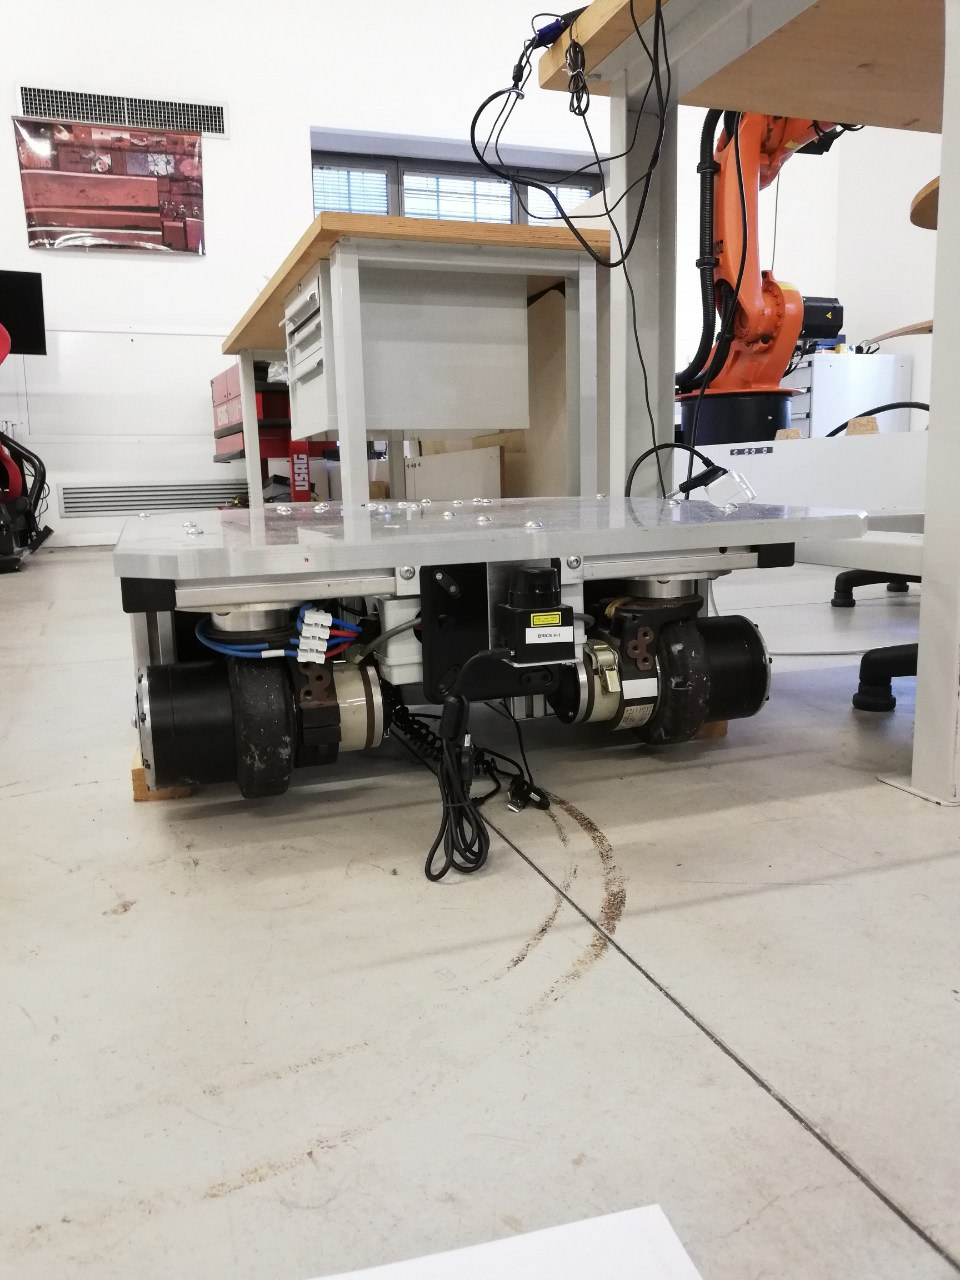
\includegraphics[width=0.5\textwidth]{Immagini/BaseRobotica.jpg}
	\caption{Base robotica addetta alla movimentazione}
	\label{fig:BaseRobotica}
\end{figure}

\begin{figure}
	\centering
	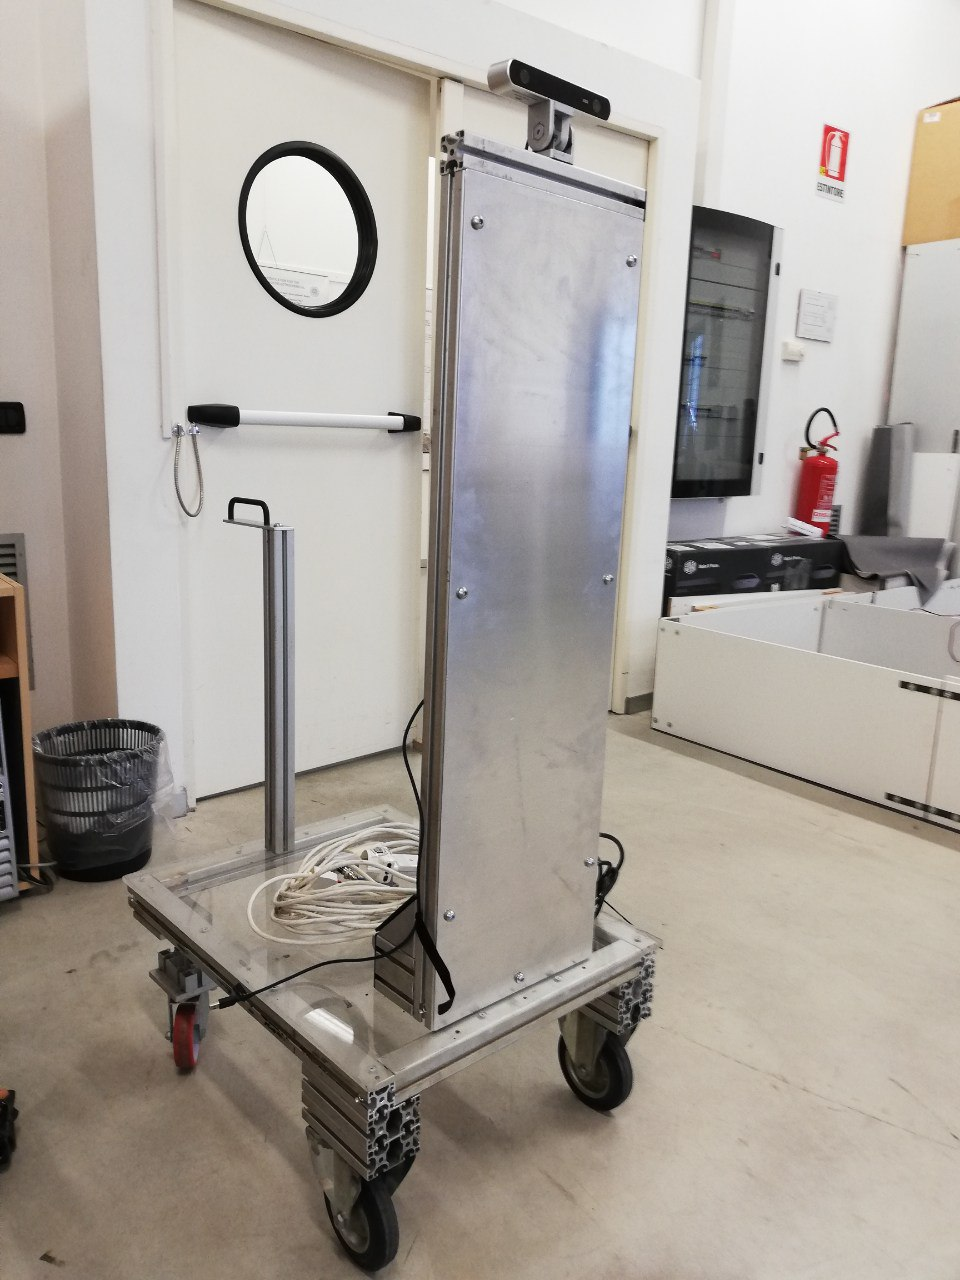
\includegraphics[width=0.5\textwidth]{Immagini/SupportoCamera.jpg}
	\caption{Base verticale sulla quale andare ad inserire la camera}
	\label{fig:SupportoRialzato}
\end{figure}

\section{SAL - Stato avanzamento lavori}
\begin{itemize}
	\item Analizzato codice Out-Of-Box del progetto dello scorso anno
	\begin{itemize}
		\item Il codice preso non aveva main: creato
		\item Compresa struttura pub/sub
		\item Analizzati topic/nodes pubblicati
	\end{itemize}
	\item Cambio camera. Perchè? Prestazioni scarse al variare della luce
	\item Nuova camera --> ueye cam
	\item Fatta funzionare nuova camera
	\begin{itemize}
		\item Demo (programma già fornito con la camera)
		\item Ros --> utilizzato file debug-launch (inserire caratteristiche che la camera fornisce quando parte lo script).
	\end{itemize}
	\item Scelta la posizione della camera: verticale inclinata e non orizzontale
	\item Progetto A.A. utilizza formule vecchie
	\item Problema CPU consuming (problema intrinseco della camera)
	\item Memory problem --> risolto con \textit{free}
	\item Doppie maschere: frecce di due colori
	\item Aggiunte queste features:
	\begin{itemize}
		\item Gaussian blur
		\item Brightness
		\item Erosion - Dilatation
	\end{itemize}
	\item Fatta erosione solo sulle frecce vicine (quelle nella metà inferiore del frame), mentre invece, le frecce nella metà superiore non vengono erose ma solo dilatate.
	\item Problema inizializzazione che mostrava rettangoli bianchi su alcune immagini intermedie nelle maschere
	\item Aggiunta distanza tra centri con tracciamente linea
	\item Prendiamo la freccia più vicina e analizziamo i dati relativi solo a questa freccia: supponendo che tutte le frecce siano uguali, è ovvio che l'area maggiore è quella della freccia più vicina (TODO: da mettere come giustificazione del codice che scriveremo)
\end{itemize}

Per creare grafi della struttura del codice ROS vedi \href{http://wiki.ros.org/rqt} e comando rqt.